\newpage

\section{Auswertung} 

\subsection{\textgamma -Absorptionskurven}

\begin{align*}
    \intertext{Durchgeführt wurde die Nullmessung ohne einen Absorber.
    Die Messung liefert}
    \text{gemessene Zeit t} = 900\,\unit{\second}\,,\\
    \text{Anzahl der Wechselwirkung N} = 959 \pm 30\,,\\
    \text{Aktivität}\,\, \text{A}_{\text{0}} = ( 1,07 \pm 0,03 )\,\frac{1}{\unit{\second}}\,.
    \intertext{Gemessen werden die Aktivitäten mit der jeweiligen Zeit.
    Die Aktivitäten werden von der Aktivität der Nullmessung abgezogen.
    Gemessen wird für Blei und Eisen. 
    Die Messwerte befinden sich in Tabelle \ref{Tabelle1} und \ref{Tabelle2}.
    Die Aktivität wird dann gegen die Dicke in einem halblogarithmischen Diagram abgetragen und über lineare Regression wird der Absorptionskoeffizient nach (\ref{1}) bestimmt.
    Mit Hilfe der Formel (\ref{5}), multipliziert mit der Formel (\ref{3}), ergibt sich der Compton-Absorptionskoeffizient $\mu_{\text{com}}$.
    Die Regressionen befinden sich in Abbildung \ref{Abbildung6} und \ref{Abbildung7}. }
\end{align*}

\begin{table}[H]
    \centering
    \caption{Messwerte zur Bestimmung des Absorptionskoeffizienten von Eisen.} 
    \label{Tabelle1}
    \begin{tabular} {c  c  c  c}
        \toprule
        {$\text{Dicke d} \mathbin{/} 10^{-3}\unit{\meter} $} &
        {$ \text{Zeit t} \mathbin{/} \unit{\second} $} &
        {$ \text{Zählrate N} $} &
        {$ \text{Aktivität} (\text{A} - \text{A}_{\text{0}}) \mathbin{/} \frac{1}{\unit{\second}} $} \\
        \midrule
        5  & 100 & 9163  \pm 95  & 90,56 \pm 0,92 \\
        5  & 100 & 8972  \pm 94  & 88,65 \pm 0,90 \\
        10 & 100 & 7654  \pm 87  & 75,47 \pm 0,77 \\
        10 & 200 & 14528 \pm 120 & 71,57 \pm 0,36 \\
        15 & 100 & 6383  \pm 79  & 62,76 \pm 0,64 \\
        15 & 200 & 11735 \pm 108 & 57,61 \pm 0,29 \\
        20 & 200 & 10022 \pm 100 & 49,04 \pm 0,25 \\
        20 & 300 & 14662 \pm 121 & 47,80 \pm 0,16 \\
        25 & 200 & 8358  \pm 91  & 40,72 \pm 0,21 \\
        30 & 300 & 10428 \pm 102 & 33,69 \pm 0,12 \\
        35 & 300 & 8000  \pm 89  & 25,60 \pm 0,09 \\
        40 & 300 & 6565  \pm 81  & 20,81 \pm 0,08 \\
        \bottomrule
    \end{tabular} 
\end{table}

\begin{figure}[H]
    \centering
    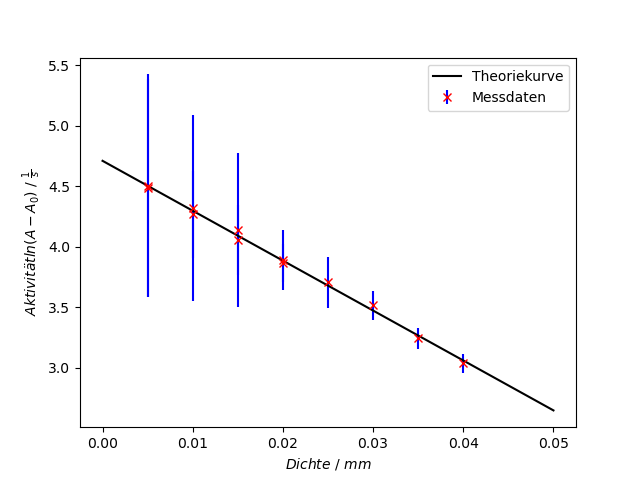
\includegraphics[height=80mm]{bilder/1.png}
    \caption{Ausgleichsrechnung von Eisen.\label{Abbildung6} }
\end{figure}

\begin{align*}
    \intertext{Daraus folgt}
    \text{negative Steigung} \equiv \text{Absorptionskoeffizient}:\,\,\,\,\, \mu = ( 41,28 \pm 0,82 )\,\frac{1}{\unit{\meter}}\,, \\
    \text{y-Achsenabschnitt} \equiv \text{Anfangsaktivität}:\,\,\,\,\, \text{A}_{0} =  ( 4,71 \pm 0,01 )\,\frac{1}{\unit{\second}}\,, \\
    \mu_{\text{com}} = 56,8\,\frac{1}{\unit{\meter}}\,.
\end{align*}

\begin{table}[H]
    \centering
    \caption{Messwerte zur Bestimmung des Absorptionskoeffizienten von Blei.} 
    \label{Tabelle2}
    \begin{tabular} {c  c  c  c}
        \toprule
        {$\text{Dicke d} \mathbin{/} 10^{-3}\unit{\meter} $} &
        {$ \text{Zeit t} \mathbin{/} \unit{\second} $} &
        {$ \text{Zählrate N} $} &
        {$ \text{Aktivität} (\text{A} - \text{A}_{\text{0}}) \mathbin{/} \frac{1}{\unit{\second}} $} \\
        \midrule
        1  & 100 & 10049 \pm 100 & 99,42 \pm 1,00 \\
        10 & 100 & 4283  \pm 65  & 41,76 \pm 0,43 \\
        12 & 100 & 3127  \pm 55  & 30,20 \pm 0,33 \\
        15 & 100 & 2390  \pm 48  & 22,83 \pm 0,26 \\
        17 & 100 & 1932  \pm 43  & 18,25 \pm 0,22 \\
        20 & 200 & 3061  \pm 55  & 14,23 \pm 0,09 \\
        22 & 200 & 2666  \pm 51  & 12,26 \pm 0,08 \\
        25 & 200 & 1990  \pm 44  & 8,88  \pm 0,07 \\
        30 & 300 & 2216  \pm 47  & 6,32  \pm 0,04 \\
        32 & 400 & 2208  \pm 46  & 4,45 \pm 0,03 \\
        35 & 400 & 1978  \pm 44  & 3,87  \pm 0,03 \\
        40 & 500 & 1787  \pm 42  & 3,34 \pm 0,02 \\
        \bottomrule
    \end{tabular} 
\end{table}

\begin{figure}[H]
    \centering
    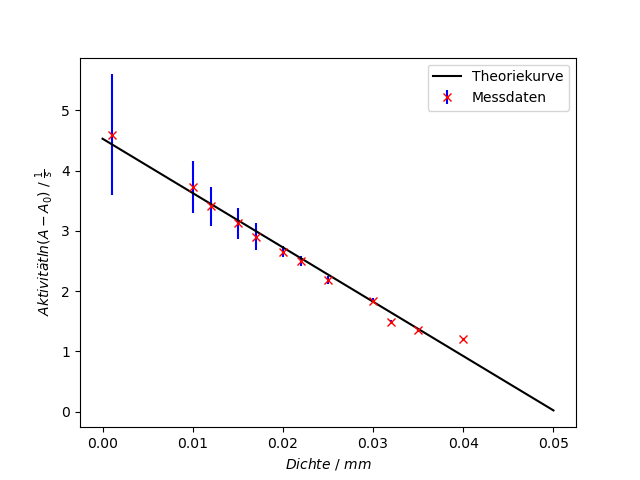
\includegraphics[height=80mm]{bilder/2.png}
    \caption{Ausgleichsrechnung von Blei.\label{Abbildung7} }
\end{figure}

\begin{align*}
    \intertext{Daraus folgt}
    \text{negative Steigung} \equiv \text{Absorptionskoeffizient}:\,\,\,\,\, \mu = ( 90,21 \pm 3,42 )\,\frac{1}{\unit{\meter}}\,, \\
    \text{y-Achsenabschnitt} \equiv \text{Anfangsaktivität}:\,\,\,\,\, \text{A}_{0} =  ( 4,53 \pm 0,08 )\,\frac{1}{\unit{\second}}\,, \\
    \mu_{\text{com}} = 68,2\,\frac{1}{\unit{\meter}}\,.
    \intertext{Die Werte liegen über bzw. unter dem gemessenen Wert.
    Es ist daher anzunehmen, dass noch zusätzlich der Photoeffekt beteiligt ist.}
\end{align*}

\subsection{\textbeta -Absorptionskurve}

\begin{align}
    \intertext{Aufgenommen wird die $\beta$ Absorptionskurve von Aluminium. 
    Daraus bestimmt wird die Maximalenergie des verwendeten $\beta$-Strahlers (\text{Tc}). 
    Die Kurve wird in zwei lineare Bereiche zerlegt oberhalb und unterhalb von $\text{R}_{\text{max}}$. 
    Erneut wird die Aktivität gegen die Dicke in einem halblogarithmischen Diagram aufgetragen. 
    Die ersten vier Messungen werden dem ersten Abschnitt zugeordnet und restlichen dem zweiten Abschnitt.
    Die letzte Messung wird in der Auswertung nicht beachtet und die Werte befinden sich in Tabelle \ref{Tabelle3}. 
    Geführt wird eine lineare Regression mit $\text{A}_{1}$, $\text{A}_{2}$, $\text{B}_{1}$ und $\text{B}_{2}$ mit der Geradengleichung}
    \text{y} = \text{A}_{\text{i}}\text{x} + \text{B}_{\text{i}} \,\,\,\,\, (\text{i} = 1,2)\,, \notag
    \intertext{zu sehen in der Abbildung \ref{Abbildung8}.
    Berechnet wird der x-Wert ($\text{R}_{\text{max}}$) des Schnittpunktes mit}
    \text{R}_{\text{max}} = \frac{\text{B}_{2} - \text{B}_{1}}{\text{A}_{1} - \text{A}_{2}}\,. \label{11}
\end{align}

\begin{table}[H]
    \centering
    \caption{Messwerte zur Bestimmung der Gesamtenergie des $\beta$-Strahlers-} 
    \label{Tabelle3}
    \begin{tabular} {c  c  c  c  c}
        \toprule
        {$\text{Dicke d} \mathbin{/} 10^{-6}\unit{\meter} $} &
        {$ \text{Zeit t} \mathbin{/} \unit{\second} $} &
        {$ \text{Zählrate N} $} &
        {$ \text{Aktivität A} \mathbin{/} \frac{1}{\unit{\second}} $} &
        {$ \text{R} \mathbin{/} \frac{\unit{\kilo\gram}}{\unit{\meter}^2} $}\\
        \midrule
        \text{ohne Absorber}  & 100 & 55000 \pm 234 & 550   \pm 1,00 & - \\
        100                   & 150 & 5775  \pm 75  & 38,50 \pm 0,26 & 0,27 \\
        125                   & 200 & 1916  \pm 43  & 9,58  \pm 0,06 & 0,33 \\
        $(153 \pm 0,5)$       & 250 & 2317  \pm 48  & 9,26  \pm 0,05 & 0,41 \\
        $(160 \pm 1)$         & 300 & 1787  \pm 42  & 5,95  \pm 0,03 & 0,43 \\
        $(200 \pm 1)$         & 350 & 875   \pm 29  & 2,50  \pm 0,03 & 0,54 \\
        $(253 \pm 1)$         & 400 & 380   \pm 19  & 0,95  \pm 0,02 & 0,68 \\
        $(302 \pm 1)$         & 450 & 332   \pm 18  & 0,73  \pm 0,02 & 0,81 \\
        $(338 \pm 5)$         & 500 & 360   \pm 18  & 0,72  \pm 0,02 & 0,91 \\
        $(400 \pm 1)$         & 550 & 354   \pm 18  & 0,64  \pm 0,01 & 1,08 \\
        $(444 \pm 2)$         & 600 & 354   \pm 18  & 0,59  \pm 0,01 & 1,19 \\
        $(482 \pm 1)$         & 650 & 454   \pm 21  & 0,71  \pm 0,01 & - \\
        \bottomrule
    \end{tabular} 
\end{table}

\begin{figure}[H]
    \centering
    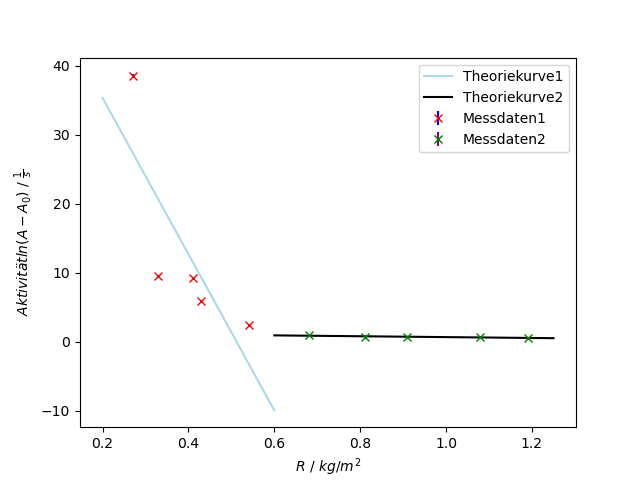
\includegraphics[height=80mm]{bilder/3.png}
    \caption{Absorptionskurve von Technetium 99. \label{Abbildung8} }
\end{figure}

\begin{align*}
    \intertext{Die gelieferten Koeffizienten lauten}
    \text{Steigung Teil 1:}\,\,\,\,\,\,\text{A}_{1} = ( -113,2 \pm 48,0 )\,\frac{1}{\unit{\meter}}\,, \\
    \text{Steigung Teil 2:}\,\,\,\,\,\,\text{A}_{2} = ( -0,62 \pm 0,14 )\,\frac{1}{\unit{\meter}}\,, \\
    \text{Y-Achsenabschnitt Teil 1:}\,\,\,\,\,\,\text{B}_{1} = ( 57,90 \pm 19,50 )\,, \\
    \text{Y-Achsenabschnitt Teil 2:}\,\,\,\,\,\,\text{B}_{2} = ( 1,31 \pm 0,13 )\,. \\
    \intertext{Somit folgt}
    \text{R}_{\text{max}} = ( 0,49 \pm 0,01 )\,\frac{\unit{\gram}}{\unit{\centi\meter}^2}
    \intertext{und mit der Formel (\ref{10}) für die Gesamtenergie}
    \text{E}_{\text{max}} = (1,13 \pm 0,02 )\cdot 10^{6}\,\text{eV}\,.
\end{align*}